\title{Connecting green space supply and demand: modeling the walkable environment of European cities}
\author{Benjamin Labohm}
\documentclass[10pt]{article}
\usepackage{geometry}
\geometry{a4paper, top=25mm, left=20mm, right=20mm, bottom=25mm,
headsep=10mm, footskip=12mm}
\setlength{\parindent}{0em} 
\usepackage{setspace}
\onehalfspacing
\usepackage{url}
%\usepackage{microtype}
\usepackage{natbib}
%\usepackage{subcaption}
\usepackage[english]{babel}
%\usepackage{multirow}
\usepackage{booktabs}
\usepackage{graphicx}
%\usepackage{lscape}
%\usepackage[toc,page]{appendix}
\begin{document}
\emergencystretch 3em
\onecolumn

{\center
\vspace*{5cm}
{\Huge Connecting green space supply and demand: modeling the walkable environment of European cities}
\par\bigskip
\Large{
\textbf{Master's thesis}\\
Humbold-Universit\"at zu Berlin

Geography Department
\\
Benjamin Labohm

Mat. Nr.: 
545609
\vfill
}
}
\large{


Supervisors: \\
Prof. Dr. Dagmar Haase

Humbold-Universit\"at zu Berlin

Geography Department\\


Dr. Manuel Wolff

Humbold-Universit\"at zu Berlin

Geography Department \\

Berlin, 15.07.2022
}

\newpage
\normalsize
\tableofcontents
\newpage
\listoffigures
\newpage

\twocolumn[{\centering{\huge Connecting green space supply and demand: modeling the walkable environment of European cities\par}\vspace{3ex}
	{\large Benjamin Labohm*\par}\vspace{2ex}
	\today\par\vspace{4ex}}
\textit{\small{*Geography Department, Humbold-Universit\"at zu Berlin, Rudower Chaussee 16, 12489 Berlin}} \\
\smallbreak
\hrule 

\vspace*{.5cm}

\textbf{Abstract}

In an increasingly urbanized world, peoples’ access to green spaces is crucial. We used network characteristics to analyze the walkable environment – the connecting area between green space demand and supply – of European cities. To make the workflow replicable for future analysis, we used open source data and software. Our results reveal a mismatch in … . Future research should focus on … .

\vspace*{.5cm}

\hrule

\par\vspace{2ex}]



\vspace{.5cm}

\normalsize


\section{Introduction}
%Part1: Accessibility to UGS
In the Anthropocene, rapid urbanization takes place globally. 55\% of the global population were living in cities by 2018 and 68\% are projected to do so in 2050.
A growing urban population depends increasingly on urban ecosystems \citep{Elmqvist.2021, UN.2019}.
Ecosystems supply ecosystem services (ES) which are critical to human well-being \citep{Fisher.2009}.
Living in proximity of urban green spaces (UGS) can help alleviate the impacts of climate change on and aging urban population, as well as improve overall public health in cities \citep{Kabisch.2021, Kabisch.2021b}.
Thus, having access to UGS can enhance urban inhabitants’ quality of life \citep{Poelman.2018}.
Likewise, the United Nations have agreed to provide universal access to public green spaces by 2030 in Sustainable Development Goal 11.7 \citep{UN.2017}.

In Europe, 74\% of the population are living in cities \citep{UN.2018}.
Here, the population pressure on UGS might be amplified by the compact city paradigm, which is popular among European city planners: A more compact city can result in shorter traveling distances but also in more overcrowding effects (Commission of European Communities, 1990; Burton.2003, Wolff.2019).
Accordingly, more people living in proximity to and benefitting from an UGS also increase the pressure on its ecological functions \citep{Wolff.2019}.
In order to detect such mismatches in green space supply and demand and to provide equal access to UGS, mapping UGS accessibility is key \citep{Larondelle.2013}.

The walkable environment – the space in between urban dwellers and UGS – not only affects the quality of ES and, thus, the accessibility of UGS \citep{Syrbe.2012}.
Availability of UGS in walking distance can improve overall public health and increase the resilience of city dwellers \citep{Kabisch.2021,Richardson.2013}.
A proper modeling of UGS accessibility must, therefore, put emphasis on modeling the walkable environment of a city \citep{Wolff.2019}.
Yet, easy to use and open source tools for comparatively modeling the walkability of European cities are lacking \citep{Kabisch.2016}.

%Part 2: State of the art
Availability and accessibility of UGS in Europe have been analyzed and compared in multiple studies.
In their 2016 paper, Kabisch et al. carried out an assessment of green space availability in 299 EU cities. They used a population grid of 1 km² and land use data (urban atlas) to calculate the population within a buffer distance of UGS \citep{Kabisch.2016}.
The use of Euclidean (direct) distance in accessibility analysis has been found to underestimate spatial distances and to overestimate the provision of UGS in contrast to using network distance, though \citep{Sander.2010, Moseley.2013}.
In 2016, the Joint Research Center (JRC) of the European Union developed an indicator for areas that are served by UGS in European cities. In their analysis, the authors used a 10 m² resolution land use data grid and a 100 m² population mosaic and a network-based approach \citep{Pafi.2016}.
In another analysis from 2018, the JRC used urban atlas data and a street network to assess the area that urban dwellers can reach in a walking distance of 10 minutes. Their analysis also resulted in an area per population measure on a city level \citep{Poelman.2018}.
Wolff and Haase looked into the connection between green space supply and residential density in 905 European cities. They found a strong link between residential density, population size and location of the cities \citep{Wolff.2019}.
Further studies have developed methods to account for problems associated with fixed catchment sizes by using variable catchment approaches \citep{Luo.2012}.

In a 2021 paper, Wolff coupled the population pressure and proximity perspectives by applying network characteristics. In his analysis, he found two promising indicators, the Detour Index (DI) and the Local Significance (LS) \citep{Wolff.2021}.
The DI is a measure of the efficiency of a route taken to reach a goal \citep{Barthelemy.2018}.
Hence, the DI can be used to model barriers that people have to overcome on their way to UGS \citep{Wolff.2021}.
The LS is a simple measure to describe the relevance of different edges of a network \citep{Esch.2014}.
With a little modification, the LS can be utilized to model use-intensity of those edges connecting population demand with UGS. As a consequence, LS might serve as a spatial indicator for overuse of UGS \citep{Wolff.2021}.

Previous research did rarely account for the mutual dependencies of supply and demand, or did it put the focus on the walkable environment \citep{Syrbe.2017}.
Using fixed distances for assessing green space accessibility might lead to numerical quantities instead of focusing on the location of the mismatch between ES supply and demand \citep{Higgs.2012, Syrbe.2017}.
Furthermore, we saw mostly one perspective being used to assess green space accessibility (provision, population pressure or proximity).
But a high provision of UGS in a city, for example, does not necessarily indicate an equal or adequate distribution of UGS \citep{Poelman.2018}.

In addition to the previous points, the mentioned studies, if on a larger scale, were carried out on a coarse resolution (Kabisch et al. 2016, European Commission 2016).
A higher resolution can reveal spatial patterns at a finer scale enabling targeted intervention while also reducing uncertainties that are introduced by e.g. a population grid or a city block aggregation as in urban atlas data \citep{Barthelemy.2018, Esch.2014}.
Achieving a high resolution on a large scale can be challenging, though, since freely available and comparable datasets are scarce \citep{Feltynowski.2018, Dworczyk.2021}.

All things considered, knowledge about green space accessibility is important for planning and decision making and mapping the capacity, flow and demand of ES in urban areas has been found to facilitate urban planning \citep{Baro.2016}.
Improving the modeling of the walkable environment with a combination of population pressure and proximity aspects of green space accessibility might prove promising to detect mismatches between UGS supply and demand \citep{Biernacka.2019, Biernacka.2020}.
Finally, municipalities across European countries still provide a mixture of different indices for measuring green space supply and demand (Kabisch et al. 2016).
Comparing cities can provide a basis for better understanding of urban processes, though \citep{Wolff.2020}.
Yet, there is no easy-to-handle and comparable tool using a high resolution on a European scale with publicly available data and software.


\subsection{Conceptualization}
The availability of UGS can be defined by the “amount of green area in a defined distance to where urban residents live” \citep{Kabisch.2016}.
Having actual access to UGS might be limited by additional factors, though. 
The physical accessibility, for example, can be limited by fences, opening hours of an UGS, or the detours people have to take to reach them. 
Additionally, accessibility may be limited by perceived overcrowding effects through population pressure \citep{Kabisch.2016, Wolff.2020b}.
As use intensity can influence ES, it can create a mismatch between supply and demand \citep{Syrbe.2017}. 

Approaches that accounted for the supply and demand aspects of ES have usually postulated a population that is close to the places of ES origin. 
Since ES are rarely consumed by humans at the same place where they are produced by the ecosystem, we distinguish service providing areas (SPA) and service demanding areas (SDA). 
Service providing areas (SPA) represent the supplying side, the spatial unit where the ES are generated \citep{Syrbe.2012, Dworczyk.2021}.
In cities, UGS supply for example the cultural ES of recreation for residents \citep{Dickinson.2017}.
Service demanding areas (SDA) embody the places where the potential demand for ES arises, e.g. the places where people live. In the case of UGS in an urban environment, residential areas or buildings are an example for SDA \citep{Dworczyk.2021}.

In order to account for physical and perceived barriers to green space access, we have to take a look at the space between SPA and SDA, the service connecting areas (SCA).
SCA can be used to show the flow of ES between SPA and SDA areas \citep{Syrbe.2012, Dworczyk.2021}.
Regarding the scenario of UGS in cities, SCA are the walkable environment, i.e. the routes residents take to benefit from the ES in their neighborhood \citep{Syrbe.2017}.
Consequently, the SCA in this case are the walkable street network of a city.

Three perspectives have been used in past studies to model the SCA for UGS: The proximity, provision and pressure perspectives.
The proximity perspective considers the space between supply and demand, e.g. the walking distance between people’s homes and the UGS, thus highlighting the SCA. 
A proximity perspective is necessary to account for barriers and other characteristics of the network. \citep{Higgs.2012, Wolff.2021}.
Furthermore, green space proximity measures have been found to be among the most important factors influencing perceived accessibility, especially for minority groups \citep{Ibes.2015, Wang.2015}. 
The widely used green space provision perspective models the flow from green area to buildings, thus, focusing on UGS provision (area / person).
Secondly, the less often used population pressure perspective describes the flow from residential buildings (i.e. the population) to the UGS.
The focus here is on the pressure of the residents on an UGS or their demand for green areas (person / area) \citep{Kimpton.2017}.

%Part 3: Objectives
Modeling the walkable environment of European cities by including the three perspectives mentioned above and using a network characteristics approach.
We want to answer the questions:

    1.) What does a modeling approach look like that estimates the walkability between green space supply and demand in cities based on high resolution data? 
    
    2.) How to incorporate publicly accessible data and open source software in order to allow i.) a reproduction over time (e.g. with more recent data), and ii.) comparative approaches covering a large sample of cities.
    
    3.) How can easily understandable and applicable indicators be used in order to support urban planning in detecting mismatches between demand and supply?
    
The objectives that we derived from these questions are i.) to develop a modeling approach that applies walkability indices, ii.) to compare the results on a European scale, and iii.) to implement the indices by showing possible use cases for city planners.



\section{Methods and Data}
\begin{figure*}[t!]
\centering
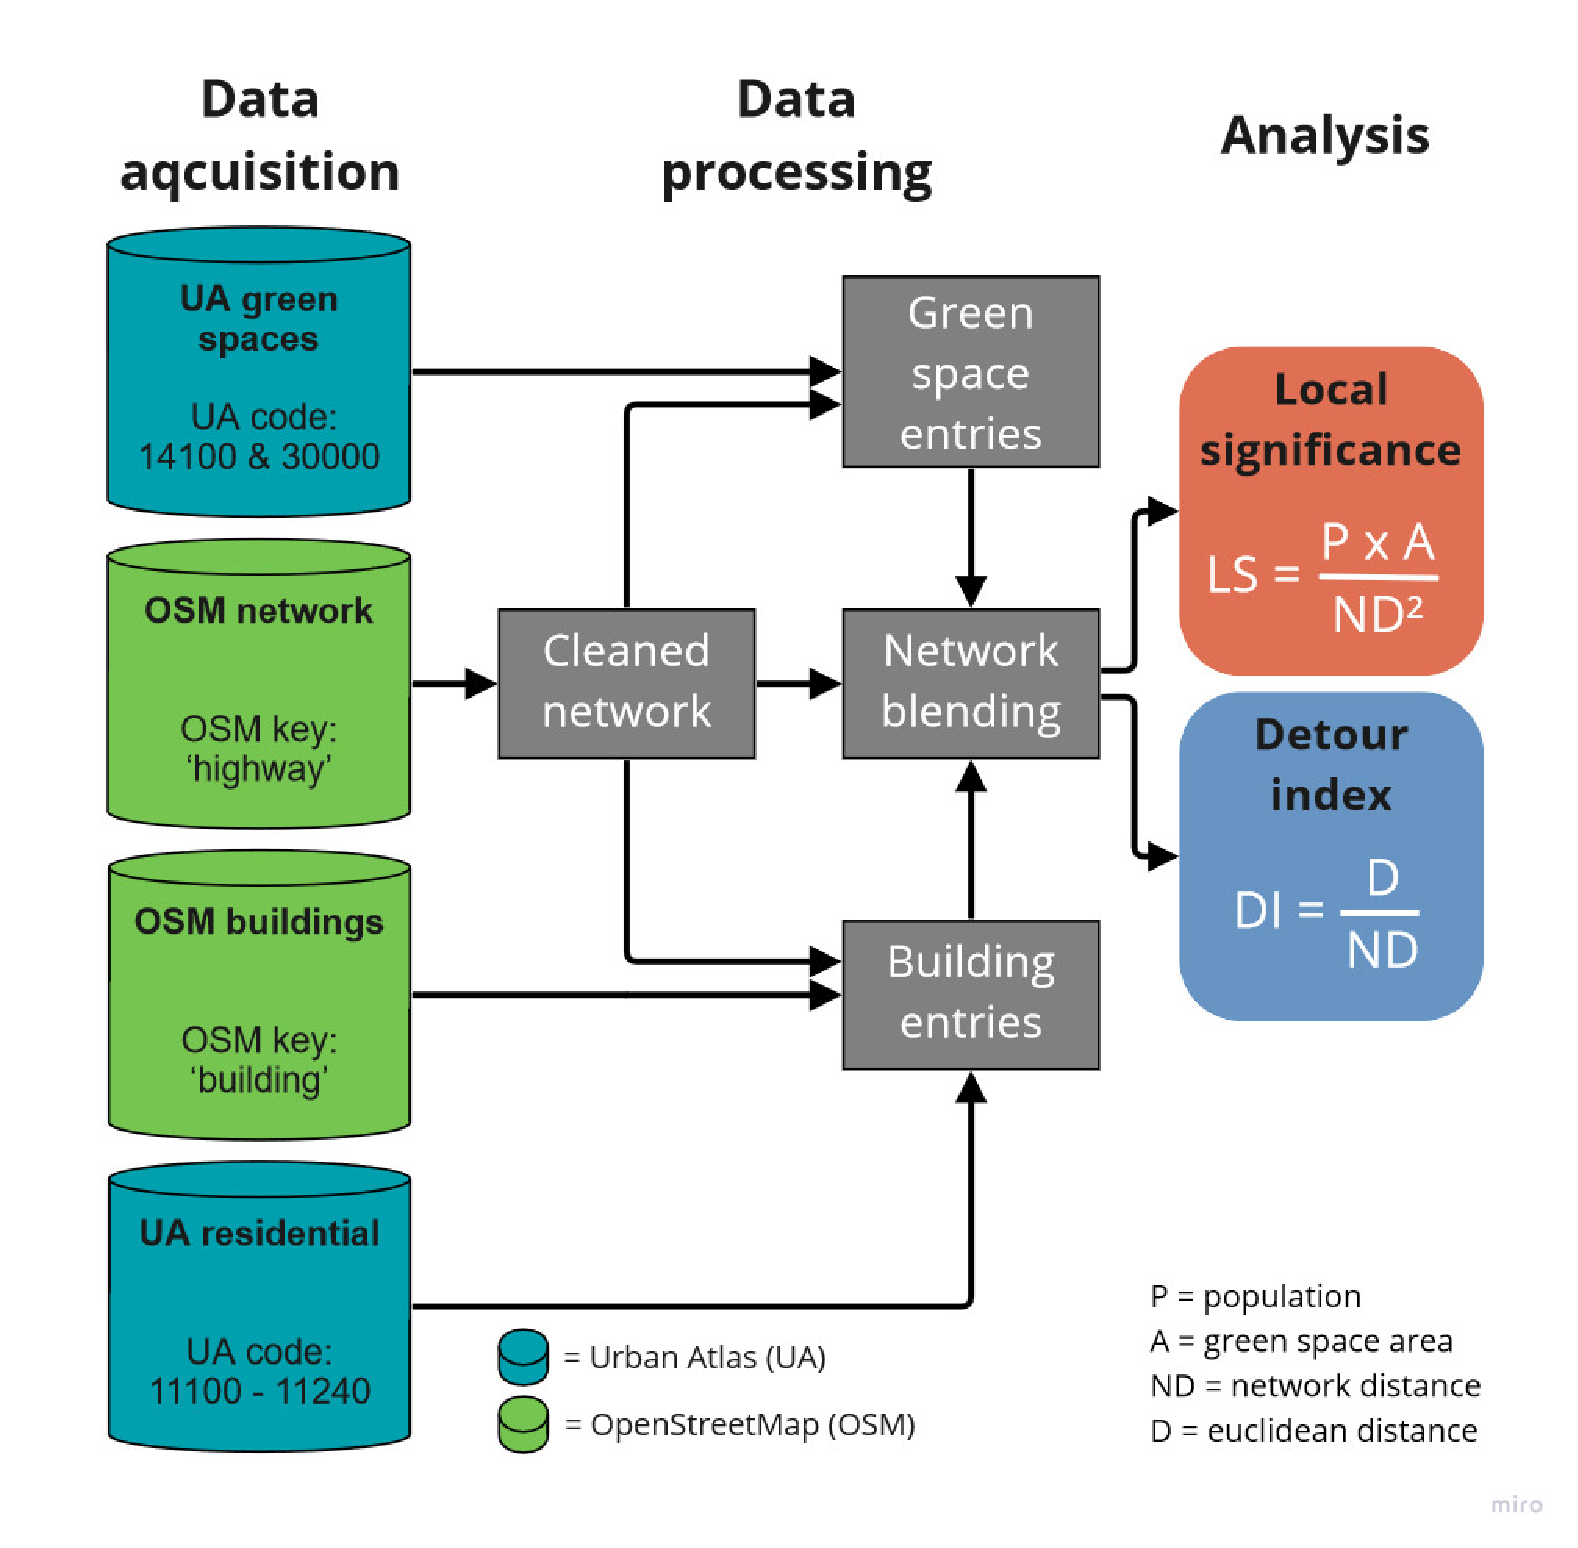
\includegraphics[width=0.6\textwidth]{2-2_md-flowchart.pdf}
\caption{Workflow of data aquisition, processing and analysis (short version). For an exhaustive version of the workflow see appendix 1a.}
\label{fig:flowchart}
\end{figure*}

\subsection{Study region}
We applied our analysis to 832 European cities.
To account for the ability of city dwellers to leave their city if they live in proximity to a city border, we included UGS from a buffer of 1 km surrounding the city boundary \citep{Wolff.2020}.
The city delineation stems from the Urban Audit dataset of the European Union \citep{EuropeanComission.2022}.

\subsection{Data}
For the analysis of the walkable environment of European cities, we needed available and comparable data on public green spaces and residential buildings and their respective entry points.
Additionally, the analysis required information on the population living in each residential building and a network that connects the buildings with the green spaces.
We aimed to incorporate publicly accessible data and open source software in order to allow i.) reproduction (e.g. with more recent data) and ii.) comparative approaches covering a large sample of cities.
We used Urban Atlas (UA) 2018 and OpenStreetMap (OSM) as our main data sources.
All analysis was carried out and tested in R 4.1.3 using RStudio version 1.4.1717 and are made available on the GitHub repository www.github.com/blabohm/MA
To ensure the best possible coverage, we downloaded the latest version possible of OSM (April / May 2022).

Urban Atlas (UA): UA is a land use / land cover (LULC) product from the Copernicus program of the European Union.
The 2018 UA version provides Europe-wide comparable data for 788 Functional Urban Areas with more than 50.000 inhabitants.
It represents 17 urban and 10 rural LULC classes with a MMU of 0.25 and 1 ha, respectively.
In addition to the spatial data, UA contains information on the population for the residential land use classes.
Since Copernicus does not offer an API, we downloaded the latest UA version available at the time of this study (c13) by hand.

OpenStreetMap (OSM): OSM is a community-based project that provides free geospatial data.
The OSM community seeks to create a database of the entire planet that is free and editable.
For the analysis we downloaded the OSM data with the identifiers ‘building’ and ‘highway’.

Since OSM is a community-based mapping service, the latest version of OSM data is expected to have the most information.
We acquired the OSM data via the OSM API, which we accessed via a custom-made tool that heavily relies on the R package ‘osmdata’.
For information on the OSM download tool see Appendix 1c.

\subsection{Data processing}
Street network: The network, in this analysis, represents the walkable environment of a city, which connects the entry points of the UGS with those of the residential buildings.
To acquire information on the street network of a city, we downloaded OSM data with the identifier ‘highway’, which represents all linestrings in the OSM database that are associated with streets and paths.
To secure comparability across European countries, we used all OSM highway classes, except for the class ‘highways’ as not being suitable for walking.
Linestrings identified with the string ‘highway’ represent motorways which are reserved for motorized use only.
To ensure network connectivity and reduce overlap, we cleaned the resulting network following the tutorial on network data pre-processing and cleaning by Lucas van der Meer (\cite{vanderMeer.2019}, https://luukvdmeer.github.io/sfnetworks, May 2022).
Further information on the network pre-processing and cleaning steps can be found in Appendix 2a.

Residential buildings: The following analysis requires information on a cities’ residential buildings, their entry points and on how many persons inhabit each building.
We filtered the OSM ‘building’ polygons for residential buildings.
We only kept those OSM buildings whose centroids were contained inside of urban atlas residential areas (UA class code starting with: 11).

Residential building entries: To detect building entries, we first calculated the centroids of each building.  
Centroids had to satisfy the constraint, that the point has to lie inside the polygon \citep{Pebesma.2022}.
We snapped the centroids to the closest point on the cleaned street network and assumed the resulting points to be the building entries.

Population per building: To assign each OSM building a reasonable population count, we used a simple area weighting disaggregation approach \citep{Li.2007}.
The UA dataset provides information on population mostly on a city block level.
We disaggregated this data to the building level by distributing the population proportionally to a buildings base area.
This workflow follows the assumption, that the building structure, and thus the population per base area inside one city block is similar.
For buildings that were contained inside UA residential polygons that erroneously did not have population values, we used the mean population per square-meter of the corresponding UA residential class in the city.

Green spaces: The last data point required for the analysis is information on publicly accessible UGS and their entry points.
We filtered the UA data for the classes ‘green urban areas’ (code 14100) and ‘forests’ (code 31000) to ensure that all green spaces that are used in the analysis are publicly accessible.
All green spaces in the UA dataset come with information on area, which we double checked for consistency.

Green space entries: To detect green space entries, we intersected the outline of the UA green spaces with the cleaned network.
Furthermore, we applied different buffer sizes to the green space polygons as sensitivity analysis.
We used the resulting points as entry points of the green spaces for the further analysis.
In case a green space did not receive any entry points, we incrementally increased the buffer sizes.
Further information on the method and the validation / sensitivity analysis can be found in Appendix 2c.

Network blending: In the process of network blending, the entry points of the residential buildings and the UGS (now called ‘nodes’) are being ‘blended’ into the network.
During this process, the lines (now called ‘edges’) will be broken at every node location.
The node location now represents the new starting / ending points of the newly created edges.
For more detailed information on this process see Appendix 2d.

\subsection{Analysis}
%Analysis to achieve Objective 1:
Our first objective was to develop a modeling approach that applies the Detour Index (DI) and Local Significance (LS) walkability indices.
For computational considerations, we limited the catchment area around each building to 500 meters network distance.
We calculated the Detour Index (DI) and the Local Significance (LS) index for each UGS inside the city core plus a buffer of 1 km.
We accounted for the maximum walking distance by calculating both indices for the residential buildings within a network distance of 500 m between a building entry and the nearest entry point of a UGS.

Detour Index (DI):  The DI is an indicator of barriers in a network.
It accounts for the efficiency of the routes that residents take on their way to the nearest UGS \citep{Wolff.2021}. The DI combines the Euclidean distance, i.e. the direct connection between two points, with the network distance \citep{Esch.2014}

Where DI is the Detour Index, D is the Euclidean distance between points i and j, and ND is the network distance between the points i and j.
In the case of this analysis, the two points are the entry points of a residential building and the nearest entry point of a UGS.
The DI can assume values between 0 and 1.
A DI value of 1 represents a straight line between building entry and UGS entry, while a DI value closer to 0 means that the inhabitants of the building have to take a sub-optimal route to the nearest UGS.
If one building has access to several UGS within a network distance of 500 m, we decided to use the mean DI value.

Local Significance (LS): The LS is usually used as an indicator of edge importance in a network analysis \citep{Esch.2014}.
We use a modified version from Wolff 2021 as an indicator of how many people have access to an UGS.
The LS also accounts for the size of an UGS as well as the distance between people’s homes and the UGS entries \citep{Wolff.2021}

Where LS is the Local Significance, p is the population of building i, A is the area of UGS j and ND is the network distance between the entry points of building i and UGS j.
This indicator can assume infinite values.
A higher population and area, as well as a lower network distance lead to higher LS values.
We attached the LS values to each segment (edge) of the path between building and UGS entries.
We summed the LS values of overlapping paths from multiple buildings, leading to higher values on higher frequented edges.
A more detailed summary on index building can be found in Appendix 3.

To demonstrate application possibilities of the indices, we visualized the DI and LS values for the area surrounding the Lene-Voigt-Park (LVP) in Leipzig.
The city of Leipzig is the largest city in Saxony, Germany. After a massive population loss in the 1990s, the city faced a major regrowth since 2012. Rising population numbers led to increased pressure on the open spaces of the city.
The LVP was a former train station area and has been out of use since 1942.
In the 2000s, it was converted to a public park and is fully open since 2004 \citep{StadtLeipzig.2022}.
Its diverse history and the population dynamic make the LVP an interesting test case for the demonstration of our results.
Since LS values tend to grow exponentially, we chose to use a logarithmic scale for visualization.

%Analysis to achieve Objective 2:
In our second objective, we wanted to compare the indices on a European level and assess in which cities the OSM data availability would facilitate our analysis.
%European comparison
For comparing the distribution of DI values in the European countries, we plotted the DI against the relative cumulative population in each city.
We aggregated the results to country level for easier visualization.
Furthermore, we mapped the percentage of people in a city that have a DI of 0.8 or higher.
To compare the LS values across European cities, we used the cities’ average of the summed LS values at the green space entries per UGS. 
%OSM data coverage
We assessed the OSM data coverage for 834 European cities.
We did so by computing the percentage of UA residential polygons that are covered by at least one OSM building polygon.
As a compromise, we used a threshold of 85\% OSM coverage (at least 85\% of the UA residential Polygons have to contain at least one OSM building polygon) for the comparison of our results across European cities.

%Analysis to achieve Objective 3:
The final objective was to implement the two indices we developed to demonstrate possible use cases for city planners.
To describe the impact of changes in different model parameters, we tested three different scenarios and calculated the change of the index values to the base model.

Alternative 1 – Unlimited access: In the first scenario we demonstrated how the LS and DI indicators change if all barriers obstructing access to the LVP were removed.
To model unlimited access, we distributed hypothetical entry points every 5 meters on the network surrounding the LVP and applied the walkability indices to the changed conditions.

Alternative 2 – Green space development: In the second scenario we investigated the impact of a development of the green spaces surrounding the LVP to residential buildings.
We assumed the following green spaces in the north of the LVP to be developed to high density residential buildings: Reudnitzer Park, Staphaniplatz, and the green space between Täubchenweg, Perthesstraße and Gerichtsweg.
To implement this scenario, we converted the former green space entry points to building entries.
We multiplied the size of the parks by the 95th percentile of the population per square meter value derived from the urban atlas high density residential class in the surrounding two kilometers.
We distributed the outcome uniformly across the former green space entries and applied the two walkability indices.

Alternative 3 – Population increase: In the third scenario we modeled a population increase in the residential areas surrounding the LVP.
For each residential building in a distance of 2 km to the LVP, we increased the population value to the 95th percentile of the respective urban atlas residential class.
We then applied the DI and LS indices to the changed conditions.
Alternative 4 – Ensemble scenario: In the final scenario we applied the changes from the unlimited access, the green space development and the population increase scenarios and gathered them in one ensemble model. 



\section{Results}

%Results
%1. Applying walkability indices

    • Figure 1: The network colors depict the cumulative LS. A higher LS value is depicted by a darker red color, representing i.) more people taking this path, ii.) the people taking this path are living in closer proximity to the green space, and / or iii.) the path is leading to a larger green space. Since the LS values are cumulative, a higher value might also mean more paths from different buildings overlapping (See Appendix … for further information). The building colors represent average DI calculated for all green spaces in a network distance of 500 meters from a building. The dark blue the color of a building is, the closer to one the DI value, the more direct can its residents travel to the closest green spaces. The opposite is the case if the color tends towards orange. 

In this section, we present the results of applying the two walkability indices to the test case, the Lene Voigt Park (LVP) in Leipzig, Germany.
Figure Xa displays the local significance (LS) values that we calculated for the city of Leipzig, Germany.
The map shows the area east of the city center (top right corner of the map). 
In the center of the map, highlighted with a darker green, is located the LVP. 
Other green spaces are depicted in a lighter green, buildings and the network in white and gray, respectively.
Lower LS values are displayed in blue shades, higher values in red shades.

Due to the high density of green spaces and residential buildings in the area, an overall high level of LS values can be observed.
In general, LS values tend to grow towards green space entry points – i.e. higher LS values can be observed in closer distance to UGS.
Due to the cumulative nature of our LS representation, this effect symbolizes street segments with the potential for overcrowding.
Furthermore, high LS values are associated with direct connections between parks and residential buildings.
The highest LS values can be found at park entries adjacent to streets which connect UGS to areas with high population, indicating street segments that are highly visited for routes towards UGS. 
The eastern part of the LVP close to the Riebeckstraße is a good example for this (marker A on the map). 
Here, we find high LS values at those parts of the streets that lead to the residential areas in the north, east and south-east.
At the same time, we see that the Riebeckstraße in this area is actually a bridge with two Tram and two car lanes and few possibilities for crossing (see picture …). 
This circumstance is not represented in the street segment´s LS values.
Furthermore, the Josephinenstraße (marker B) which connects the center of the LVP to the next larger park in the south, the Friedenspark (marker C), displays high LS values.
On the other hand, we can make out lower LS values at streets with residential buildings that are close to the cut-off threshold of 500 meters distance to the nearest green space.
For example, in the southeast of the map, in many streets, the blue shade is getting brighter with each street segment until it switches over to red shades.
With each building entry, more inhabitants are expected to take these routes towards the nearest green space.
This increases the LS values of the street segments.

Figure Xb displays the detour index (DI) east of the city center of Leipzig.
Higher DI values are depicted in blue shades, lower ones in red shades.
High DI values can be found at buildings that are located at streets which lead directly to a green space entry. 
Along these streets there are straight formations of buildings with high DI values as can be seen in the south of the LVP. 
In contrast, there occur clusters of low DI values in areas where larger detours have to be taken to reach a park entry. Such areas can be found in the northeast of the map. 
Furthermore, we can observe low DI values at buildings that are close to several UGS but whose routes towards one or more UGS are inefficient.
Some buildings that are directly adjacent to one UGS, but have to take small detours to the nearest green space entry point, also show low DI values.
Lastly, we see that there are buildings close to UGS with high DI values but that have to cross larger streets or other obstacles to reach the green space entry point.


%2. Comparing walkability indices

Figure 2 Percentage of urban atlas residential class polygons that contain at least one OpenStreetMap building polygon. Red colors represent a higher coverage. Yellow and blue colors represent lower share of covered polygons.

Here, we present the results of the OSM data coverage assessment and, later, compare the two walkability indices across Europe.
Figure x depicts the OSM coverage, i.e. the relative share of UA polygons that are covered by at least one OSM building polygon. 
Most cities in central Europe – in particular in Poland, the Czech Republic, Austria, Northern Italy, Switzerland, France, Belgium and the Netherlands – exhibit a very high OSM coverage of nearly 100 percent. 
In the UK, northern Spain and the southeast of Europe, we see more cities with an OSM coverage of around 50\%.
In Portugal and the south of Spain few cities express an OSM coverage above 50\%, and most cities are around 25\% OSM coverage.
In figure x we see two exemplary cities – Vienna as an example for a high OSM coverage and Lisbon as an example for a low OSM coverage.
The city of Vienna, Austria is a prime example for a high OSM coverage with 98.7\% of the UA residential building polygons covered by at least one OSM building.
A source of error explaining a fraction of the imperfect coverage in most cities are misclassified UA polygons (see Appendix 1b).
In another share of UA polygons, the population values might have been so small that none of the OSM buildings received a population count, so they got filtered out during the data cleaning process (see Appendix 2b).
In contrast, in Lisbon, Portugal 55.6\% of the UA polygons are covered by OSM buildings. 
As we see in figure …a, most of the low coverage can be explained by a lacking digitalization of buildings in the OSM dataset.
Additionally, the OSM building coverage in Lisbon is declining with higher distance from the city center.
Where OSM buildings are present, the workflow of generating LS and DI indices was functional.
On the other hand, large parts of the residential areas of Lisbon have no OSM coverage and, thus did not get index values.
This lack of DI values for a large part of the population would complicate a comparison with other cities that have a more complete coverage.
Also, comparing the LS values could prove unreliable, even though we use the average value at green space entry for the above analysis.
Missing residential buildings in the service area of green spaces would lead to LS values that might be lower than expected.
Due to these inconsistencies, we decided to exclude all cities with an OSM coverage of less than 85\% from our analysis.
Most of Europe’s capital cities feature a high OSM coverage and by choosing a threshold of 85\%, we only had to exclude 5 of them from our analysis (Lisbon, Athens, Budapest, London and Madrid).  

Figure 3 Top: share of population with DI values of 0.8 or greater (in cities with OSM coverage > 85\%, n = 533). Bottom: DI values per share of population.

In this section we compare the DI and LS indices in 533 European cities with an OSM coverage of 85\% or higher (see previous section).
To compare the DI of European cities, we will have a look at the cities’ DI per relative cumulative population.
For the example of the LVP, a share of roughly 45\% of the population in the surrounding area has a DI of 0.8 or higher:

%DI_plot_small

In figure x (DI MAP) we demonstrate this share of population for each city.
Here, we can observe a clustering of cities with mid- to high shares of population with DI values above 0.8 in northern and central European countries.
This cluster consists especially of cities in the Netherlands, Belgium and Germany, as well as the western parts of Poland and the Czech Republic.
In France, the UK, Italy and the eastern part of Poland, we see a larger share of cities with a lower percentage of population with DI values greater than 0.8.
Most Balkan countries, as well as Ireland have no cities with a > 20\% share of population in the highest DI segment.
As we can see in figur­­­­e x, the distribution of DI values plotted against the cumulative, relative population varies strongly across countries.
The ending points of the lines show the percentage of people with green spaces in a network distance of 500 meters. 
The slopes of the lines indicate how direct the inhabitants of a country can travel to the green spaces they have access to.
On the top end there are mostly northern and central European countries where more than 85\% of the urban population can reach green spaces in 500 meters network distance.
On the lower end there are mostly southern and south eastern European countries where less than 30\% of the population or less live in 500 meters network distance of green spaces.
It is notable, that on both ends of the spectrum, the sample size is limited to only a few cities (top: FI = 3, SE = 5, LU = 1, bottom: AL = 2, XK = 1, RS = 3, RO = 5).
Yet, there are countries with large city samples and a high percentage of population reaching green spaces in 500 meters network distance, like Germany (126 cities, 73\%) or Poland (68 cities, 69\%). 
Additionally, there are countries with large city samples and a lower percentage of people in proximity to green spaces like France (84 cities, 58\%) and Italy (56 cities, 57%).
In France, for example, we see a higher share of population with a more direct access to UGS in the north-eastern part of the country and a lower one towards the south-western part.
Generally, a curve that has a late onset and a steep slope means that more people have a more direct route to the nearest green spaces and vice versa. 
An example for this would be Finland, where about 32\% of the urban population have an DI of more than 0.8. 
On the contrary, the curve of Norway has an early onset and a lower ending point, resulting in a smaller share of people (23\%) having a DI in the highest 0.2 margin.

Figure 4 (top): Mean LS at green space entry points per city (color) and LS coverage – i.e. percent green spaces in a city that have been reached by inhabitants (size). (bottom): Mean LS values at green space entry points per city. Aggregated by country.
The average LS values at green space entry of the European cities also show a large variation.
For example, in figure X (LS MAP) we can observe above average LS values at the green space entries in mid- to southwestern Germany.
According to our results, in these areas the street segments at the UGS entries are highly visited, UGS are large and / or the population lives close to the UGS. 
In contrast, most of the cities in France or at the eastern coast of Italy feature rather low LS values.  
In Poland or the Netherlands, we find a mixed picture of cities with higher and lower LS values at green space entry.
In figure x we see the LS values aggregated on a country level. 
Every point that is plotted behind the box-plots represents the average LS value at green space entry of one city.
Accordingly, we see that the differences in the number of cities where our analysis was feasible vary substantially between countries.
At the bottom and top ends of the chart, there are countries where relatively few cities are included in the final analysis, like Greece, Luxembourg or Norway.
From the countries with a larger share of cities that were eligible for our analysis, Italy has the largest spread of LS values.
Like France and the Netherlands, Italy’s mean LS at UGS entry is at the line indicating the lowest 25\% of cities, while the mean values of Germany and Poland are in the middle of the 25\% and the 75\% lines.
Again, a high average LS at UGS entry might indicate more people at the UGS entries, larger UGS and / or population living closer to UGS.


%3. Implementing walkability indices

In this section we want to demonstrate how local planners can use the two walkability indicators that we applied before.
Therefore, we return to the example of the LVP as outlined in section X.1.
We explore three potential alternatives in which we reshape the built environment as an expression of applied planning tools.
In each alternative, we alter one of the core variables that are used to calculate LS and DI.
In the first alternative, “unlimited access”, we assume that the LVP can be accessed from all around the park.
For the second alternative, “densification”, we selected a number of UGS north of the LVP and replaced them with residential buildings.
In the last alternative, “population growth”, we assume a certain increase in residents in the area surrounding the LVP.

 Alternative 1 – Unlimited access 
Figure? Delta values for local significance (left) and detour index (right). Streets and buildings that expressed no change are not colored. An increased LS is mapped in red, a decrease in blue. Increasing LS values depict street segments that are higher visited. An increasing DI is mapped in blue, a decrease in red. Higher DI means that the trajectories from a building to the nearest UGS entry have become more efficient. The top two maps show the unlimited access alternative. 

In the first alternative we demonstrate how the LS and DI indicators change if all barriers obstructing access to the Lene-Voigt-Park (LVP) were to be removed.
We do so by assuming a park entry every 5 meters on the network surrounding Lene-Voigt-Park.
As can be seen in figure \ref{•}, a decrease in LS values occurs on all streets that are adjacent to the LVP. 
On most of the remaining streets, we observe an increased LS.
Thus, according to our model, removing the barriers along the edges of the LVP would result in less crowded streets surrounding the park, which may be a desirable effect for city planners.
On the other hand, more people could reach the LVP, increasing the overall amount of people traveling through net network and towards the park. 
Accordingly, removing entry barriers could also be a pull factor for an UGS.

Figure \ref{•} shows the change of the DI values in the first alternative.
When the DI of a building increases, the routes towards the nearest UGS have become more direct, representing a facilitated access to the nearest UGS for the residents of the building.
Overall, we mostly observe minor changes of DI values (delta-DI < 0.1) when providing unlimited access.
We filtered out any delta-DI values that were smaller than +/-0.05 to place emphasis on the more significant changes.
It appears as though the change of DI values is mostly limited to buildings that are either very close to the park or that were not reachable before, but are now inside the threshold network distance of 500 meters.
A few buildings adjacent to the eastern part of the LVP express an increase larger than 10%. 
A larger area to the northeast and smaller areas to the east and south of the center of the LVP show a minor increase of DI values. 
These buildings may now be able to take a more efficient trajectory towards the LVP.
In the northwest of the map we see a cluster of buildings that seems to have gained access to the LVP via a direct path, which increased their DI values.
Contrary, in the southeast there is a couple of buildings that have gained access as well, but on a less direct path.
For these buildings the DI values decreases, meaning the average trajectories towards the nearest UGS have become less efficient.

Alternative 2 – Densification
In the second alternative we intended to see how the indices behave if the green spaces in the city blocks north of the LVP were to be developed into residential areas.
To apply these changes, we switched the former park entries into building entries and distributed among them population according to the former park’s size.
Figure x-c shows that overall, most of the LS values appear to decrease substantially. 
Since the UGS disappeared, the trajectories of the people that traveled to them have disappeared as well, leading to decreased LS.
Only on the paths connecting the newly built residential areas to the LVP and the former Johannes-cemetery in the west (marker A) can we see a substantial increase of LS values.
Overall, the reduction of the number of parks in the area seems to have a larger effect on the LS-index than the increase in population due to the newly “constructed” residential buildings. 

In Figure X-d we see DI values mostly increasing in the area. 
Especially the buildings along the Heinrichstraße (marker B) that leads from the center of the LVP north experience a substantial DI increase.
Again, a higher DI means more efficient routes to the nearest parks.
Some areas in the east and north of the map express a decrease of DI values, representing less efficient trajectories towards the nearest UGS.
South and west of the LVP we observe a mixed picture of minor de- and increases.
The five green spaces that we intended to change into residential areas are comparatively small and, thus, “hard to reach”.
Taking them out of the equation seems to leave the surrounding buildings with more efficient trajectories towards the larger parks.

Alternative 3 – Population increase
The third alternative is designed to demonstrate how a population increase would affect the DI and LS indices.
In this alternative, we assumed for each residential building a population increase to the 95th percentile of the population per area according to its urban atlas residential class.
Since we did not change the locations of any green spaces or building entries, the DI index did not change, either.
As we can see in figure x, the delta-LS is positive in the entire area.
In contrast to the other alternatives, changes are now scattered across the entire map, since we also applied the population growth all buildings in the area.
In this alternative, we see a similar pattern as in the basic LS map (see figure x). 
LS tends to grow larger, the closer a street is to one of the large parks, specially along those streets, where the population flows from multiple areas combine on their way towards the UGS.
For example, we can observe high LS values between the LVP and the Friedenspark in the south of LVP.
The further away a street is from the larger parks, the lower the increase of the LS.
Close to LVP we now observe a large cluster with high LS values in the west.
If we have a look at the population data that is attached to the residential buildings, we can see that the area in the northwest of the LVP has several buildings with very high population (see appendix for larger version of the image).
Most of these buildings can reach the LVP only via the entry point at the northwest, which causes the high LS values in this area. 

Alternative 4 – Ensemble model
In the final alternative, we applied all the changes of the previous three alternatives at once. 
The joint effects of removing barriers, developing the green space in the north and a population increase can be seen in figures x a and b.
Figure x a, shows that the change of the LS index is mostly influenced by the population increase and the green space development alternatives.
Due to the population increase, we see a general increase of LS, except for those streets that experience a decrease of LS due to the removed green spaces.
This makes the changes of the LS appear more diffuse than in the other alternatives.
Similar to the population increase alternative, we see a large area with high LS increase in the northwest of the LVP.
In this alternative we can simultaneously observe the effects of the population increase and the unlimited access alternatives.
The nearest entry point for the area with the high population residential buildings in the northwest has been shifted to the northernmost corner of the LVP in contrast to the third alternative.
As we can observe in figure x b, change of DI is restricted to those buildings that either reached one of the now developed green spaces before or that can reach the LVP through one of the new entry points.
In the fourth alternative we can still see an overall increase in DI from removing the small and hard-to-reach green space in the north of the LVP.
Also, the mixed effects from removing the entry barriers to the LVP can still be observed in the south or the northwest of the LVP. 
For both, LS and DI, the overall changes in this alternative appear more gradual than e.g. in the densification scenario and are most apparent where we applied intense constructional changes.  



\section{Discussion}


\section{Conclusions}

\bibliographystyle{apalike}
\bibliography{bibliography}
%\bibliographystyle{apalike}

\onecolumn
\newpage
Erkl\"arung

Ich erkl\"are, dass ich die vorliegende Arbeit nicht f\"ur andere Pr\"ufungen eingereicht, selbst\"andig und nur unter Verwendung der angegebenen Literatur und Hilfsmittel angefertigt habe. S\"amtliche fremde Quellen inklusive Internetquellen, Grafiken, Tabellen und Bilder, die ich unver\"andert oder abgewandelt wiedergegeben habe, habe ich als solche kenntlich gemacht. Mit ist bekannt, dass Verst\"oße gegen diese Grunds\"atze als T\"auschungsversuch bzw. T\"auschung geahndet werden.

Berlin, den 12.10.2018\\

\par\bigskip
\par\bigskip

Unterschrift
\end{document}
